\documentclass[tikz,border=10pt]{standalone}
\usepackage{amsmath}
\usetikzlibrary{calc,angles,quotes}
\begin{document}
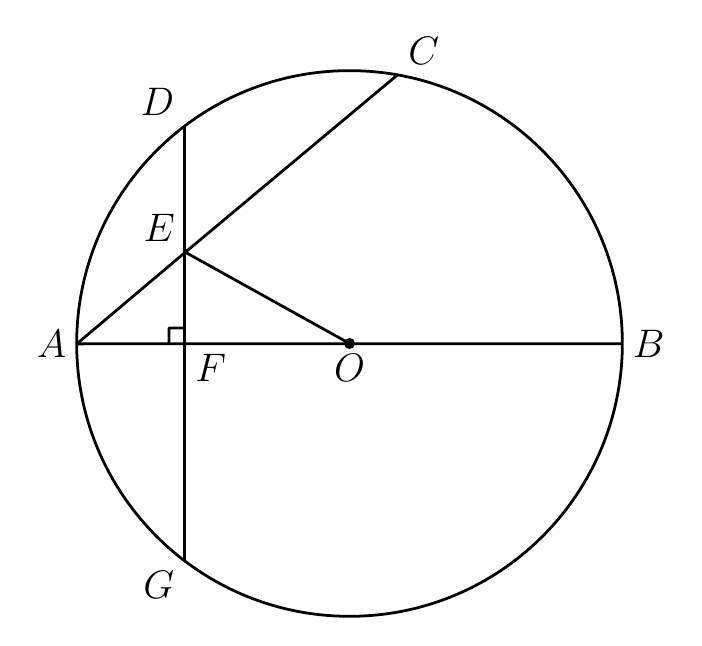
\begin{tikzpicture}[line join=round, line width=1.0pt,
  lbl/.style={font=\fontsize{14}{16.8}\selectfont}]
\coordinate (A) at (-3.487,-0.293);
\coordinate (B) at (3.442,-0.291);
\coordinate (C) at (0.589,3.125);
\coordinate (D) at (-2.115,2.478);
\coordinate (F) at (-2.115,-0.291);
\coordinate (G) at (-2.115,-3.049);
\coordinate (O) at (-0.023,-0.288);



\coordinate (E) at (-2.108,0.871);


\draw (O) circle (3.465);


\draw (A) -- (B);


\draw (D) -- (G);


\draw (A) -- (E) -- (C);


\draw (E) -- (O);


\draw pic[draw, angle radius=0.200cm] {right angle=A--F--D};


\fill (O) circle (2.000pt);


\node[lbl, left] at (A) {$A$};
\node[lbl, right] at (B) {$B$};
\node[lbl, above right] at (C) {$C$};
\node[lbl, above left] at (D) {$D$};
\node[lbl, above left] at (E) {$E$};
\node[lbl, below right] at (F) {$F$};
\node[lbl, below left] at (G) {$G$};
\node[lbl, below] at (O) {$O$};
\end{tikzpicture}
\end{document}